\section{k-Nearest Neighbors}
\label{sec: knn}

k-Nearest Neighbors is one of the simplest machine learning algorithms\footnote{kNN is also used for regression. In this note, only the use for classification is discussed.}. Lets imagine we have $N$ training examples in our feature space which are given by:

\begin{itemize}
  \item a feature vector $\vec x = (x_1, x_2, ... , x_n)$
  \item a class membership $y$
\end{itemize}

For a given vector $\vec x'$ we want to determine its membership $y'$. The idea is to look at $k$ nearest neighbors and let the majority decide - if among the $k$ nearest neighbors the most of training vectors belongs to the class $y_j$, the given vector also belongs to $y_j$. The optimal value of $k$ is unique for the problem and must be determine empirically. 

\begin{figure}

  \centering\begin{tikzpicture}

  \begin{axis}[xlabel = $x$, ylabel = $y$, xmin = -5.0, xmax = 5.0, ymin = -5.0, ymax = 5.0]
    
    \addplot[mark = *, , draw = none, color = orange] coordinates {(1,1)} node[pin=90:{\color{gray}\small$(1,1)$}]{}; 
    \addplot[mark = *, , draw = none, color = orange] coordinates {(-1,2)} node[pin=90:{\color{gray}\small$(-1,2)$}]{}; 
    \addplot[mark = *, , draw = none, color = orange] coordinates {(-2,1)} node[pin=120:{\color{gray}\small$(-2,1)$}]{}; 

    \addplot[mark = *, , draw = none, color = blue] coordinates {(-1,-2)} node[pin=270:{\color{gray}\small$(-1,-2)$}]{}; 
    \addplot[mark = *, , draw = none, color = blue] coordinates {(2,-2)} node[pin=270:{\color{gray}\small$(2,-2)$}]{}; 
    \addplot[mark = *, , draw = none, color = blue] coordinates {(-3,-1)} node[pin=270:{\color{gray}\small$(-3,-1)$}]{}; 

    \addplot[mark = *, , draw = none, color = red] coordinates {(-1,-1)} node[pin=15:{\color{gray}\small$(-1,-1)$}]{};

  \end{axis}

\end{tikzpicture}
  \caption{Two classes of points: blue and orange. The red dot represents the point to classify.}
  \label{fig: knnExample}
  
\end{figure}

\begin{table}
\begin{center}
\begin{tabular}{c | c | c}

class & coordinates & distance$^2$ \\ \hline
\color{blue}blue     & $(-3,-1)$ & $4$  \\
\color{blue}blue     & $(-1,-2)$ & $1$  \\
\color{blue}blue     & $(2,-2)$  & $10$ \\ \hline
\color{orange}orange & $(-1,2)$  & $9$  \\
\color{orange}orange & $(1,1)$   & $8$  \\
\color{orange}orange & $(-2,1)$  & $9$  \\

\end{tabular}
\end{center}

\caption{The list of distances between the red point and each training example from Fig. \ref{fig: knnExample}.}
\label{tab: knnExDist}

\end{table}

Lets consider the example presented on Fig. \ref{fig: knnExample}. There are two classes of points: blue and orange. The size of the training set is 6 (3 for each class). The red point is the one to classify (by eye it looks like it should belongs to blue points).

The distances\footnote{Actually, squares of distances are considered, as it does not affect the result, but we avoid square roots.} between the red point and each training example are presented in Tab. \ref{tab: knnExDist}. Euclidean metric was used, however, the choice of a metric is arbitrary and we could use as well Chebyshev distance, cosine similarity etc. Now, lets take a look how we classify the red point for different $k$:

\begin{itemize}
 \item[\color{blue}blue] for $k = 1$, $2$, $3$
 \item[\color{orange}orange] for $k = 5$
 \item[\color{red}tie] for $k = 4$, $6$
\end{itemize}

This was ultra-simple example to demonstrate the method, but still some conclusions can be drawn:

\begin{itemize}
  \item for binary classification $k$ should be odd to avoid a tie
  \item large $k$ does not necessary mean better results (especially when $k \sim$ training sets size)
  \item one can consider simple expansion with {\it vote weight} depending on the distance
\end{itemize}

Lets consider once again the given example, but now each point votes for a class membership with the weight given by 1 / distance$^2$, as in Tab. \ref{tab: knnExDistW}. Now, for any $k \in [1,6]$ the red point is classified as blue:

\begin{itemize}
 \item[k = 1:] {\color{blue}1.000} vs {\color{orange}0.000} 
 \item[k = 2:] {\color{blue}1.250} vs {\color{orange}0.000} 
 \item[k = 3:] {\color{blue}1.250} vs {\color{orange}0.125} 
 \item[k = 4:] {\color{blue}1.250} vs {\color{orange}0.236} 
 \item[k = 5:] {\color{blue}1.250} vs {\color{orange}0.347} 
 \item[k = 6:] {\color{blue}1.350} vs {\color{orange}0.347} 
\end{itemize}


\begin{table}
\begin{center}
\begin{tabular}{c | c | c | c}

class & coordinates & distance$^2$ & weight \\ \hline
\color{blue}blue     & $(-3,-1)$ & $4$  & 0.250 \\
\color{blue}blue     & $(-1,-2)$ & $1$  & 1.000 \\
\color{blue}blue     & $(2,-2)$  & $10$ & 0.100 \\ \hline
\color{orange}orange & $(-1,2)$  &  $9$ & 0.111 \\
\color{orange}orange & $(1,1)$   & $8$  & 0.125 \\
\color{orange}orange & $(-2,1)$  & $9$  & 0.111 \\

\end{tabular}
\end{center}

\caption{The list of distances between the red point and each training example from Fig. \ref{fig: knnExample}. The vote weight is defined as 1 / distance$^2$.}
\label{tab: knnExDistW}

\end{table}

\subsection{Separable points}
\label{sec: knnSep}

\begin{figure}
\hfill
\subfigure[Default]{\includegraphics[width=0.48\textwidth]{figures/knn_95_85_separable_default_weighted_samples.eps} \label{fig: knnSepTrainSetDef}}
\hfill
\subfigure[Distant]{\includegraphics[width=0.48\textwidth]{figures/knn_95_85_separable_distant_weighted_samples.eps} \label{fig: knnSepTrainSetDis}}
\hfill
\centering\subfigure[Overlapped]{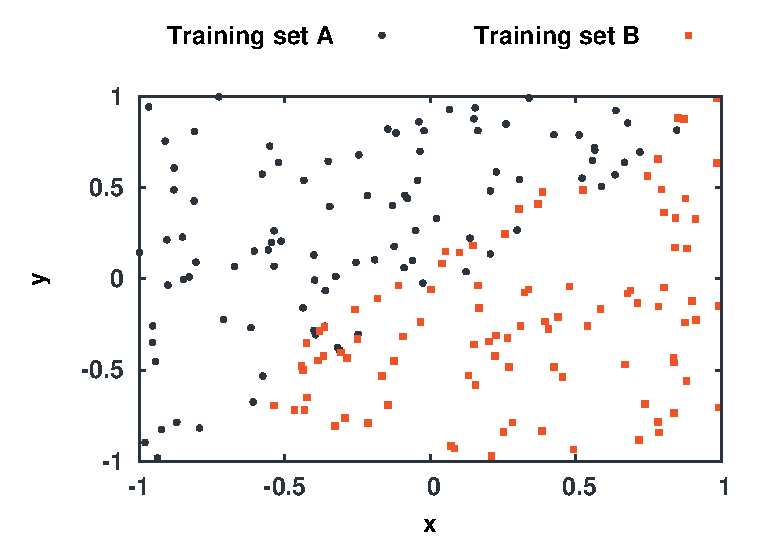
\includegraphics[width=0.48\textwidth]{figures/knn_95_55_separable_overlapped_weighted_samples.eps} \label{fig: knnSepTrainSetOvr}}
\hfill
\caption{Training sets for points separable by $f(x) = x$.}
\label{fig: knnSepTrainSet}
\end{figure}

Lets consider something defined mathematically better than {\it blue} and {\it orange}, i.e. two classes of points which can be separated linearly, e.g. by the line $f(x) = x$ as presented on Fig. \ref{fig: knnSepTrainSet} in three scenarios:

\begin{itemize}
 \item points are exactly separated by $f(x) = x$, Fig. \ref{fig: knnSepTrainSetDef}
 \item there is a small gap to make points more separated, Fig. \ref{fig: knnSepTrainSetDis}
 \item points overlap a little, Fig. \ref{fig: knnSepTrainSetOvr}
\end{itemize}

For each scenario the efficiency of kNN as a function of the size of training sets ($n$) and $k$ is checked in the following way:

\begin{enumerate}
 \item generate $n$ random points above $f(x) = x$ (training set A)
 \item generate $n$ random points below $f(x) = x$ (training set B)
 \item generate a random point
 \item find $k$ nearest neighbors of this point
 \item let them vote:
 \begin{itemize}
  \item with vote weight = $1$ (unweighted)
  \item with vote weight = $1/$distance (weighted)
 \end{itemize}
 \item repeat points 3-5 $N$ times to get good enough statistics ($N = 10^5$ for presented results, but every $100$ test points new training sets are generated)
 \item calculate the score = no. of correctly guessed points / no. of all test points
\end{enumerate}

The efficiency of kNN as a function of $k$ and $n$ can be found on Fig. \ref{fig: knnSepRes}. Clearly, weighted voting gives better results, especially for $k \sim n$. However, even unweighted kNN still gives score better than 90\%. The efficiency is almost the same when extra gap is generated between training sets (Figs. \ref{fig: knnSepResDisU} and \ref{fig: knnSepResDisW}), but it becomes much worse if training sets overlap (Figs. \ref{fig: knnSepResOvrU} and \ref{fig: knnSepResOvrW}).

\begin{figure}
\hfill
\subfigure[Default, unweighted]{\includegraphics[width=0.48\textwidth]{figures/knn_separable_default_unweighted.eps} \label{fig: knnSepResDefU}}
\hfill
\subfigure[Default, weighted]{\includegraphics[width=0.48\textwidth]{figures/knn_separable_default_weighted.eps} \label{fig: knnSepResDefW}}
\hfill
\subfigure[Distant, unweighted]{\includegraphics[width=0.48\textwidth]{figures/knn_separable_distant_unweighted.eps} \label{fig: knnSepResDisU}}
\hfill
\subfigure[Distant, weighted]{\includegraphics[width=0.48\textwidth]{figures/knn_separable_distant_weighted.eps} \label{fig: knnSepResDisW}}
\hfill
\subfigure[Overlapped, unweighted]{\includegraphics[width=0.48\textwidth]{figures/knn_separable_overlapped_unweighted.eps} \label{fig: knnSepResOvrU}}
\hfill
\subfigure[Overlapped, weighted]{\includegraphics[width=0.48\textwidth]{figures/knn_separable_overlapped_weighted.eps} \label{fig: knnSepResOvrW}}
\hfill
\caption{kNN efficiency for points separable by $f(x) = x$.}
\label{fig: knnSepRes}
\end{figure}

\begin{figure}
\hfill
\subfigure[Training sets]{\includegraphics[width=0.48\textwidth]{figures/knnWrongTrainSet.eps} \label{fig: knnWrongTrainSet}}
\hfill
\subfigure[Testing set]{\includegraphics[width=0.48\textwidth]{figures/knnWrongTrainResults.eps} \label{fig: knnWrongTrainResults}}
\hfill
\hfill
\caption{The example of the kNN classification using wrong training sets ($n = 100$, $k = 50$).}
\label{fig: knnWrongTrain}
\end{figure}

Lets take a look what happens when training sets are not uniformly distributed, as presented on Fig. \ref{fig: knnWrongTrain}. It still looks (by eye) that training sets are separated by $f(x) = x$, see Fig. \ref{fig: knnWrongTrainSet}. However, from obvious reasons some points are going to be incorrectly classified, as presented on Fig. \ref{fig: knnWrongTrainResults}.

